\section{Parameter estimation}

\begin{figure}[!htbp]
\minipage{.47\textwidth}%
\centering
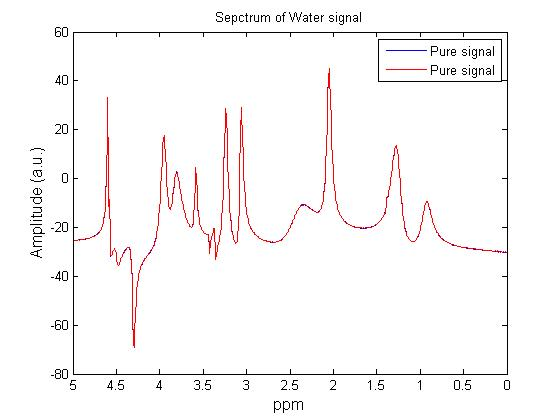
\includegraphics[width=1\textwidth]{35.jpg}
\subcaption{Spectrum of signals to be processed}
\endminipage\hfill
\minipage{.47\textwidth}%
\centering
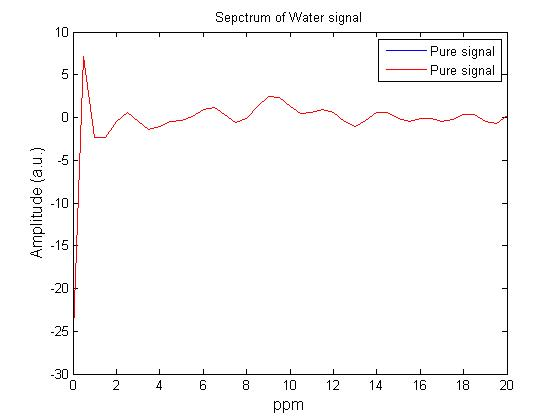
\includegraphics[width=1\textwidth]{36.jpg}
\subcaption{The signals to be processed in time domain}
\endminipage\hfill
\centering
\caption{The pure water filtered signal at model order 30 and the noisy signal coming from the superposition of the white Gaussian noise with mean zeros and the variance equal last 300 points of the water filtered signal}
\end{figure}



\begin{figure}[!htbp]
\minipage{.47\textwidth}%
\centering
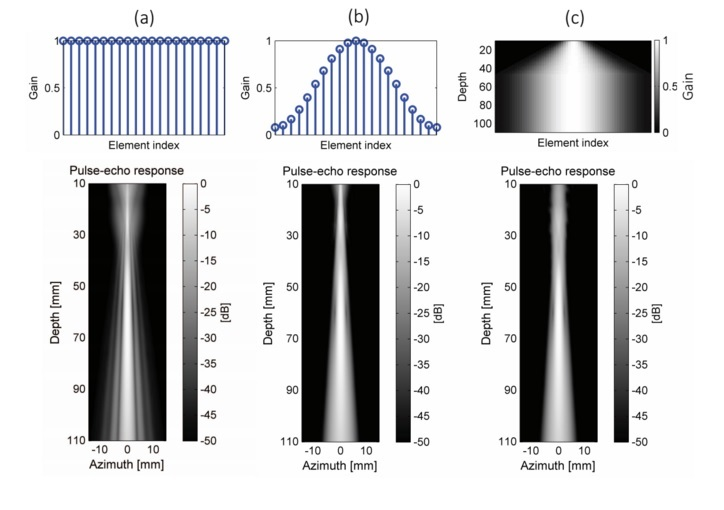
\includegraphics[width=1\textwidth]{22.jpg}
\subcaption{Reconstruction of noise free signal after hsvD, htls, htlspk estimation}\label{today1}
\endminipage\hfill
\minipage{.47\textwidth}%
\centering

\includegraphics[width=1\textwidth]{23.jpg}
\subcaption{Reconstruction of noisy signal after hsvD, htls, htlspk estimation}\label{today2}
\endminipage\hfill
\caption{Plot of the reconstructed spectrum for both the }
\end{figure}


\begin{figure}[!htbp]
\minipage{.47\textwidth}%
\centering
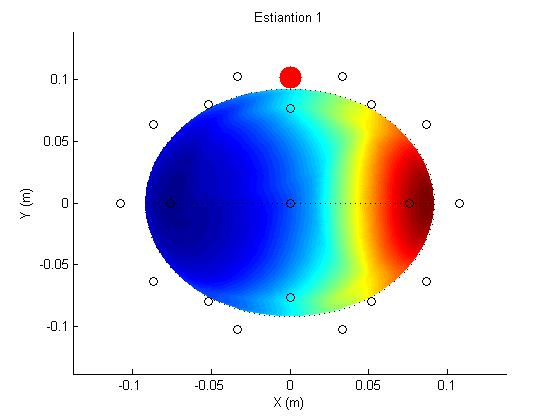
\includegraphics[width=1\textwidth]{24.jpg}
\subcaption{Residue of noise free signal after hsvD, htls, htlspk estimation}
\endminipage\hfill
\minipage{.47\textwidth}%
\centering
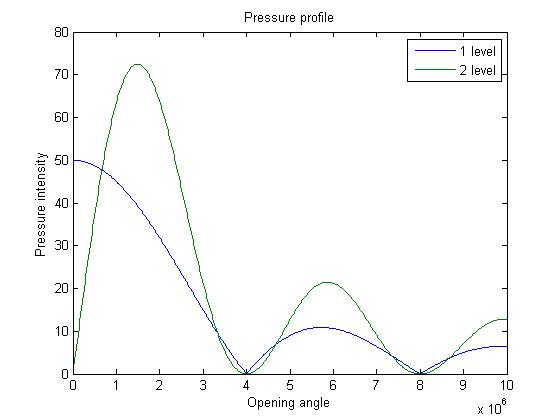
\includegraphics[width=1\textwidth]{25.jpg}
\subcaption{Residue of noisy signal after hsvD, htls, htlspk estimation}
\endminipage\hfill
\centering
\caption{The residue of both pure and noisy signals are included. This is computed as the difference between the input signal \textit{(pure or noisy)} and the outcome signal for respective method.}
\end{figure}

Using subspace methods for parameter estimation aims a very good fit between the reconstructed signal and the signal of interest. The accuracy of the method scales up, starting with the hsvD method moving into higher accuracy with htls. This is confirmed in both, SNR of the respective methods observed into the final signal and to the variance of the residue for respective signal. SNR tends to be higher contrary the variance tends to scale down, indicating a very good fit to the signal. In the figure \ref{today1} and \ref{today2} SNR values are bigger for the htls case compare to hsvD in both pure and noisy signal. In the work of \textbf{Chen et al 2011} it was possible to incorporate frequency and damping factor for the htls method. The result in the pure signal exhibit an improvement of the SNR compare to the both previous signals. Nevertheless it is still inferior compare to the htls without prior knowledge for the noisy signal case. This might outcome as a result of small inaccuracy of the prior knowledge which is incorporate subsequently arising into an less accurate results. 

Apart for the SNR  htlspkfd perform the best fit compare to both hsvd and htls in the pure signal case. Likewise, the fit tend to be less accurate in the noisy case from htlspkfd compare to htls, wherein under the same assumption. The prior values tend to be less accurate for the noisy signal consequently reflecting less accurate fit. 
However both SNR and the fit is much more accurate compare to the hsvd mode in both pure and noisy signal scenario. 
 

  

\newpage


























 \begin{table}[!htbp]
\centering
\caption{Frequency estimation \textbf{\textit{Hz}}}
\label{table:5}
\begin{tabular}{c c c c c c c c c c c c c c c c c c c c c c c c c c c c c c c } 
   \hline 

$Compo$&$HSVD$&$HTLS$&$HTLSPKFD$&$HSVD$&$HTLS$&$HTLSPKFD$\\
   \hline
$K$&$Pure signal$&$Pure signal$&$Pure signal$&$Noisy signal$&$Noisy signal$&$Noisy signal$\\
   \hline
   
   
   
   
$1$&$0.8987$&$ 0.9086$&$0.6562 $&$ 0.9081$&$ 0.9080$&$ 0.9080$\\
$2$&$0.8187$&$ 0.8071$&$ 0.5221$&$ 0.8317$&$ 0.8317$&$ 0.8321$\\
$3$&$0.6377$&$ 0.6377$&$ 0.4879$&$ 0.4122$&$ 0.4061$&$ 0.7914$\\
$4$&$0.5166$&$ 0.5166$&$-0.0128$&$ 0.2983$&$ 0.2983$&$ 0.2983$\\
$5$&$-0.0128$&$-0.0128$&$-0.0161$&$ 0.1575$&$ 0.1575$&$ 0.1575$\\
$6$&$-0.0161$&$-0.0161$&$-0.0268$&$ 0.0794$&$ 0.0794$&$ 0.0794$\\
$7$&$-0.0268$&$-0.0268$&$-0.0507$&$-0.0128$&$-0.0128$&$ -0.0128$\\
$8$&$-0.0507$&$-0.0507$&$-0.0929$&$-0.0161$&$-0.0161$&$ -0.0161$\\
$9$&$-0.0955$&$-0.0955$&$-0.0955$&$-0.0268$&$-0.0268$&$ -0.0268$\\
$10$&$-0.1118$&$-0.1118$&$-0.1118$&$-0.0507$&$-0.0507$&$ -0.0507$\\
$11$&$-0.1424$&$-0.1424$&$-0.1424$&$-0.0792$&$-0.0792$&$ -0.0789$\\
$12$&$-0.1624$&$-0.1624$&$-0.1624$&$-0.0955$&$-0.0955$&$ -0.0929$\\
$13$&$-0.1706$&$-0.1706$&$-0.1706$&$-0.1118$&$-0.1118$&$ -0.0955$\\
$14$&$-0.1864$&$-0.1864$&$-0.1864$&$-0.1424$&$-0.1424$&$ -0.1118$\\
$15$&$-0.2085$&$-0.2085$&$-0.2085$&$-0.1572$&$-0.1572$&$ -0.1423$\\
$16$&$-0.2195$&$-0.2100$&$-0.2126$&$-0.1624$&$-0.1624$&$ -0.1572$\\
$17$&$-0.2913$&$-0.2913$&$-0.2913$&$-0.1706$&$-0.1706$&$ -0.1624$\\
$18$&$-0.3029$&$-0.3026$&$-0.3013$&$-0.1864$&$-0.1864$&$ -0.1706$\\
$19$&$-0.3228$&$-0.3190$&$-0.3036$&$-0.2085$&$-0.2085$&$ -0.1864$\\
$20$&$-0.3386$&$-0.3386$&$-0.3386$&$-0.2914$&$-0.2914$&$ -0.2085$\\
$21$&$-0.3547$&$-0.3598$&$-0.3408$&$-0.2982$&$-0.2982$&$ -0.2914$\\
$22$&$-0.4229$&$-0.4229$&$-0.4195$&$-0.3386$&$-0.3386$&$ -0.2982$\\
$23$&$-0.4244$&$-0.4246$&$-0.4229$&$-0.4229$&$-0.4229$&$ -0.3386$\\
$24$&$-0.4306$&$-0.4313$&$-0.4237$&$-0.4356$&$-0.4358$&$ -0.4229$\\
$25$&$-0.4358$&$-0.4358$&$-0.4358$&$-0.4391$&$-0.4390$&$ -0.4359$\\
$26$&$-0.4391$&$-0.4391$&$-0.4391$&$-0.4810$&$-0.4810$&$ -0.4390$\\
$27$&$-0.4810$&$-0.4810$&$-0.4810$&$-0.8317$&$-0.8316$&$ -0.4810$\\
$28$&$-0.5441$&$-0.5441$&$-0.5434$&$-0.9080$&$-0.9080$&$ -0.8317$\\
$29$&$-0.6182$&$-0.6240$&$-0.5449$&$-0.9559$&$-0.9558$&$ -0.9080$\\
$30$&$-0.9561$&$-0.9561$&$-0.9561$&$-0.9830$&$-0.9770$&$ -0.9560$\\
   
   

    
     \hline 

\end{tabular}
\end{table}





 \begin{table}[!htbp]
\centering
\caption{Damping estimation \textbf{\textit{Hz}}}
\label{table:5}
\begin{tabular}{c c c c c c c c c c c c c c c c c c c c c c c c c c c c c c c } 
   \hline 
$Compo$&$HSVD$&$HTLS$&$HTLSPKFD$&$HSVD$&$HTLS$&$HTLSPKFD$\\
   \hline
$K$&$Pure signal$&$Pure signal$&$Pure signal$&$Noisy signal$&$Noisy signal$&$Noisy signal$\\
   \hline 
$1$  &$3.8888$&$ 3.8888$&$ 3.8888$&$ 3.8876$&$3.8875$&$3.8881$\\
$2$&$    1.8040$&$ 0.2089$&$ 0.5232$&$ 0.6610$&$ 0.1393$&$0.1394$\\
$3$ &$   0.7106$&$ 0.1812$&$ 0.1388$&$ 0.3541$&$ 0.0581$&$ 0.0730$\\
$4$  &$  0.4398$&$ 0.1387$&$ 0.0754$&$ 0.1394$&$ 0.0543$&$ 0.0581$\\
$5$&$    0.3966$&$ 0.0579$&$ 0.0729$&$ 0.0581$&$ 0.0504$&$ 0.0546$\\
$6$ &$   0.1991$&$ 0.0543$&$ 0.0580$&$ 0.0543$&$ 0.0326$&$ 0.0504$\\
$7$  &$  0.1387$&$ 0.0498$&$ 0.0543$&$ 0.0497$&$ 0.0298$&$ 0.0328$\\
$8$&$    0.1212$&$ 0.0371$&$ 0.0498$&$ 0.0363$&$0.0253$&$0.0297$\\
$9$ &$   0.0580$&$ 0.0325$&$ 0.0372$&$ 0.0326$&$ 0.0226$&$0.0253$\\
$ 10$ &$  0.0542$&$ 0.0253$&$ 0.0324$&$ 0.0253$&$ 0.0206$&$ 0.0226$\\
$11$&$    0.0498$&$ 0.0225$&$ 0.0253$&$ 0.0226$&$0.0172$&$0.0207$\\
$ 12$ &$  0.0421$&$ 0.0207$&$ 0.0226$&$ 0.0207$&$ 0.0149$&$0.0172$\\
$13$&$    0.0372$&$ 0.0181$&$ 0.0207$&$ 0.0172$&$ 0.0133$&$ 0.0149$\\
$14$ &$   0.0325$&$ 0.0171$&$ 0.0171$&$ 0.0149$&$ 0.0070$&$ 0.0133$\\
$ 15$ &$  0.0253$&$ 0.0148$&$ 0.0149$&$ 0.0133$&$ 0.0060$&$ 0.0070$\\
$16$&$    0.0226$&$ 0.0132$&$ 0.0133$&$0.0070$&$0.0058$&$0.0060$\\
$17$ &$   0.0207$&$ 0.0115$&$ 0.0071$&$ 0.0060$&$ 0.0036$&$0.0058$\\
$ 18$ &$  0.0172$&$ 0.0095$&$ 0.0061$&$ 0.0058$&$ 0.0024$&$ 0.0034$\\
$19$&$    0.0149$&$ 0.0070$&$ 0.0056$&$ 0.0024$&$ 0.0014$&$ 0.0024$\\
$20$&$   0.0133$&$ 0.0060$&$ 0.0036$&$ 0.0022$&$ 0.0011$&$ 0.0014$\\
$21$ &$  0.0071$&$ 0.0057$&$ 0.0026$&$ 0.0018$&$ 0.0010$&$ 0.0010$\\
$22$&$    0.0061$&$ 0.0024$&$0.0023$&$0.0016$&$0.0007$&$0.0007$\\
$23$ &$   0.0060$&$ 0.0015$&$ 0.0013$&$0.0015$&$-0.0001$&$-0.0002$\\
$24$  &$  0.0057$&$ 0.0014$&$ 0.0011$&$0.0014$&$-0.0002$&$-0.0002$\\
$25$   &$ 0.0057$&$ 0.0009$&$ 0.0006$&$0.0014$&$-0.0002$&$-0.0002$\\
$26$    &$0.0024$&$ 0.0007$&$ 0.0005$&$0.0012$&$-0.0002$&$-0.0002$\\
$27$&$    0.0014$&$ 0.0001$&$ 0.0000$&$0.0008$&$-0.0003$&$-0.0003$\\
$28$&$    0.0011$&$ -0.0001$&$-0.0003$&$0.0003$&$-0.0004$&$-0.0004$\\
$29$ &$  -0.0029$&$-0.0035$&$-0.0011$&$0.0002$&$-0.0013$&$-0.0016$\\
$ 30$ &$ -0.0031$&$-0.0035$&$-0.0031$&$-0.0003$&$-0.0016$&$-0.0016$\\
    \hline 

\end{tabular}
\end{table}


 \begin{table}[!htbp]
\centering
\caption{Amplitude estimation \textbf{\textit{a.u}}}
\label{table:5}
\begin{tabular}{c c c c c c c c c c c c c c c c c c c c c c c c c c c c c c c } 
   \hline 
$Compo$&$HSVD$&$HTLS$&$HTLSPKFD$&$HSVD$&$HTLS$&$HTLSPKFD$\\
   \hline
$K$&$Pure signal$&$Pure signal$&$Pure signal$&$Noisy signal$&$Noisy signal$&$Noisy signal$\\
   \hline 
$1   $&$32.6329$&$32.6329$&$32.6329$&$32.6298$&$32.6280$&$32.6303$\\
$2   $ &$1.1981$&$ 1.1981$&$ 1.1981$&$1.2022$&$1.2014$&$1.2020$\\
$3$&$    1.0859$&$ 1.0859$&$ 1.0859$&$1.0798$&$1.1177$&$ 1.1213$\\
$4$ &$   0.9033$&$ 0.9033$&$ 0.9033$&$ 0.9037$&$0.9034$&$0.9120$\\
$5$  &$  0.8092$&$ 0.8092$&$ 0.8092$&$ 0.8112$&$ 0.8112$&$0.8266$\\
$6$&$    0.8086$&$ 0.8086$&$ 0.8086$&$ 0.8073$&$ 0.8074$&$ 0.8074$\\
$7$ &$   0.6667$&$ 0.6667$&$ 0.6667$&$ 0.6661$&$ 0.6661$&$ 0.6664$\\
$8$  &$  0.5733$&$ 0.5732$&$ 0.5733$&$ 0.5737$&$ 0.5737$&$ 0.5738$\\
$9$   &$ 0.5072$&$ 0.5072$&$ 0.5072$&$ 0.5071$&$ 0.5070$&$ 0.5072$\\
$10$    &$0.3205$&$ 0.3205$&$ 0.3205$&$ 0.3201$&$ 0.3201$&$ 0.3204$\\
$11 $   0&$.2034$&$ 0.2035$&$ 0.2035$&$ 0.2034$&$ 0.2034$&$ 0.2034$\\
$12 $   0.&$1825$&$ 0.1825$&$ 0.1825$&$ 0.1826$&$ 0.1826$&$ 0.1828$\\
$13$&$    0.1245$&$ 0.1245$&$ 0.1245$&$ 0.1205$&$ 0.0930$&$ 0.0931$\\
$14$ &$   0.0932$&$ 0.0931$&$ 0.0931$&$ 0.0930$&$ 0.0726$&$ 0.0735$\\
$15$  &$  0.0653$&$ 0.0653$&$ 0.0653$&$ 0.0657$&$ 0.0657$&$ 0.0656$\\
$16$&$    0.0439$&$ 0.0439$&$ 0.0439$&$ 0.0432$&$ 0.0432$&$ 0.0432$\\
$17$ &$   0.0192$&$ 0.0191$&$ 0.0192$&$ 0.0190$&$ 0.0189$&$ 0.0216$\\
$18$  &$  0.0099$&$ 0.0098$&$ 0.0099$&$ 0.0100$&$ 0.0100$&$ 0.0189$\\
$19$&$    0.0000$&$ -0.0001$&$ 0.0000$&$0.0020$&$ 0.0003$&$ 0.0101$\\
$20$ &$   0.0000$&$ 0.0000$&$-0.0001$&$0.0015$&$0.0003$&$0.0003$\\
$21$  &$  0.0000$&$ -0.0001$&$ 0.0000$&$0.0004$&$  0.0003$&$0.0002$\\
$22$&$    0.0000$&$ 0.0000$&$0.0000$&$0.0003$&$0.0002$&$0.0001$\\
$23$ &$   0.0000$&$ 0.0000$&$ 0.0000$&$0.0002$&$0.0001$&$0.0001$\\
$24$  &$  0.0000$&$ 0.0000$&$ 0.0000$&$ 0.0002$&$0.0001$&$0.0001$\\
$25$   &$ 0.0000$&$ -0.0001$&$ 0.0000$&$0.0002$&$ 0.0001$&$0.0001$\\
$26$    &$0.0000$&$ 0.0000$&$0.0000$&$0.0002$&$0.0001$&$0.0001$\\
$27$&$  0.0000$&$ 0.0000$&$ 0.0000$&$0.0002$&$0.0001$&$0.0001$\\
$28$&$    -0.0001$&$ -0.0001$&$0.0000$&$0.0002$&$0.0001$&$0.0001$\\
$29$   &$ -0.0001$&$0.0000$&$0.0000$&$0.0001$&$0.0000$&$0.0001$\\
$30$    &$-0.0001$&$-0.0001$&$0.0000$&$0.0000$&$0.0000$&$0.0000$\\
     \hline 

\end{tabular}
\end{table}



 \begin{table}[!htbp]
\centering
\caption{Phase estimation \textbf{\textit{Deg}}}
\label{table:5}
\begin{tabular}{c c c c c c c c c c c c c c c c c c c c c c c c c c c c c c c } 
   \hline 

$Compo$&$HSVD$&$HTLS$&$HTLSPKFD$&$HSVD$&$HTLS$&$HTLSPKFD$\\
   \hline
$K$&$Pure signal$&$Pure signal$&$Pure signal$&$Noisy signal$&$Noisy signal$&$Noisy signal$\\
   \hline 
$1$&$  353.0457$&$353.0457$&$353.9060$&$353.3338$&$353.0316$&$353.0277$\\
$2$ &$ 352.5020$&$352.5020$&$353.0457$&$353.0305$&$352.5485$&$352.5421$\\
$3$ &$ 342.7687$&$342.7687$&$352.5020$&$352.5437$&$342.7033$&$342.6403$\\
$4$  &$342.0433$&$342.0433$&$345.1340$&$342.6973$&$341.9824$&$341.9757$\\
$5$&$  329.1565$&$329.1565$&$342.7687$&$342.0679$&$329.1524$&$329.1508$\\
$6$ &$ 325.6619$&$325.6619$&$342.0433$&$329.1519$&$325.5254$&$325.5798$\\
$7$  &$313.3449$&$313.3449$&$341.2040$&$325.5312$&$313.2785$&$313.3143$\\
$8$&$  311.4413$&$282.7090$&$329.1565$&$313.2660$&$308.6737$&$309.0136$\\
$9$ &$ 307.8060$&$259.6805$&$325.6619$&$304.4009$&$304.2548$&$303.4103$\\
$10$  &$282.7090$&$256.9107$&$313.3450$&$282.7573$&$282.9388$&$282.9014$\\
$11$&$  279.4737$&$249.8693$&$296.2705$&$277.5808$&$275.9693$&$254.9584$\\
$12$ &$ 259.8489$&$227.0606$&$282.7090$&$272.2716$&$256.0013$&$249.6786$\\
$13$  &$238.4413$&$185.6412$&$243.8925$&$265.5952$&$204.8138$&$218.4549$\\
$14$&$  234.6404$&$149.5597$&$185.6412$&$212.2177$&$185.6322$&$185.6365$\\
$15$ &$ 185.6411$&$148.4096$&$168.8839$&$185.6279$&$150.1872$&$177.1757$\\
$16$  &$170.1475$&$126.3778$&$161.5672$&$150.2351$&$148.4314$&$162.9075$\\
$17$  &$149.5597$&$122.6237$&$158.7715$&$148.4255$&$147.6220$&$150.1472$\\
$18$  &$148.4096$&$119.5757$&$149.5597$&$140.8382$&$141.7136$&$148.4846$\\
$19$&$  119.5757$&$100.6838$&$148.4096$&$119.7685$&$122.7716$&$125.3330$\\
$20 $&$ 100.6838$&$97.9307$&$119.5757$&$98.5117$&$119.7707$&$120.0598$\\
$21 $ &$ 98.8727$&$74.9523$&$101.4028$&$98.4081$&$98.3968$&$98.3028$\\
$22$&$   97.9306$&$71.4598$&$100.6838$&$85.3232$&$98.3468$&$ 61.1008$\\
$23$ &$  91.5578$&$48.6633$&$97.9307$&$77.8430$&$50.5836$&$52.7016$\\
$24$  &$ 90.6754$&$29.7034$&$80.2124$&$49.8303$&$49.3632$&$49.8074$\\
$25$&$   63.3129$&$16.1521$&$48.6633$&$49.0087$&$47.8449$&$47.8806$\\
$26$ &$  51.2416$&$14.2335$&$29.7034$&$47.8570$&$36.5071$&$46.9110$\\
$27 $ &$ 48.6633$&$13.6347$&$14.2336$&$29.8902$&$29.8965$&$29.8477$\\
$28 $  &$29.7034$&$ 7.2483$&$ 4.7676$&$14.4915$&$19.1006$&$17.1431$\\
$29 $  &$14.2336$&$ 6.9159$&$ 3.9155$&$13.7611$&$17.1397$&$16.3458$\\
$30 $   &$4.7676$&$ 4.7675$&$ 3.1099$&$4.7621$&$4.7517$&$5.1473$\\
   \hline 

\end{tabular}
\end{table}  
    
    
      
\newpage
\subsection{Subspace methods for parameter estimation}
 Parameter estimation is possible via either via subspace methods, or via optimization methods.
 
 Subspace methods employs least square estimation technique for the estimation of the parameters. This is an optimization technique where the real intended value is never reached in real scenario. The lower bound of this bias estimation is outcomed from Cramer-Rao criteria. The ambiguity of this estimation increases with the number of the unknown parameter and this is even conformed from the Fisher information matrix. 
 
 
Even tough very hard to be done, it is possible to incorporate prior knowledge on the estimation this will increase the accuracy of the parameter estimation \cite{7}. The more prior knowledge we have the more accurate the estimation will be. Different types of prior knowledge has a totally different approach for their incorporation where in most of the cases is never straight forward\cite{8}.

Contrary to the optimization based methods subspace methods don't require any iterative estimation consequently the complexity in this case far better. Moreover the estimation requires no cost function to be modeled where its importance is mostly related to the number of steps towards the best result.

Subspace methods does not ensure the best estimation possible however it ensures that there is not local minimum reached, which in the optimization case this could be possible when the method does not explore the candidates globally. However via prior knowledge the CR bound is approached quite significantly\cite{7}.

The user capability to initialize the parameters of the subspace methods is very important. In case of MRS signal the number of peaks is an visual estimated. This restricted the method from being fully automatized. 

Subspace methods are very good candidate for the parameter estimation of closely spaced sinusoid thereby making them excellent method for metabolite detection in MRS \cite{9}.  

Subspace methods are very robust estimation, meaning that they will claim a good result out in best scenario whereas in the optimization method, some internal error could occur during the computation of the cost function\cite{9}.

Furthermore, subspace methods are capable for parameter estimation of multiple different signals at the same time via the extension of the existing HTLS based algorithms\cite{10}. Consequently big data could be processed simultaneously instead of a iteration over single signal in the optimization case.

Last but not least the same estimation over the same values is not ensured via subspace methods for parameter estimation. 


